\documentclass[10pt, a4paper]{article}

\usepackage[utf8]{inputenc}
\usepackage[english, spanish]{babel}
\usepackage[left=25mm, right=25mm, top=35mm, bottom=30mm, headheight=35mm]{geometry}
\usepackage{graphicx}
\usepackage{float}
\usepackage{xcolor}
\usepackage{fancyhdr}
\usepackage{hyperref}
\usepackage{setspace}
\usepackage{indentfirst}

% Syntax customization with minted package
\usepackage{minted}
\usemintedstyle{nord-darker}
\usemintedstyle[zsh]{gruvbox-light}
\setminted{
  breaklines,
  linenos,
  frame=lines,
  fontsize=\normalsize
}
\newcommand{\mts}[1]{\mintinline[style=gruvbox-light]{typescript}{#1}}

% Define background color
\definecolor{background}{HTML}{2E3440}

% Variables
\newcommand{\university}{Universidad Nacional de San Agustín de Arequipa}
\newcommand{\faculty}{Facultad de Ingeniería de Producción y Servicios}
\newcommand{\program}{Escuela Profesional de Ingeniería de Sistemas}
\newcommand{\semester}{2024 - A}
\newcommand{\course}{img/web_programming.png}
\newcommand{\topic}{img/angular.png}
\newcommand{\professor}{Carlo Jose Luis Corrales Delgado}
\newcommand{\students}{Armando Steven Cuno Cahuari\\Victor Narciso Mamani Anahua\\Jorge Luis Mamani Huarsaya}
\newcommand{\github}{https://github.com/jorghee/angular-hangman-s-game}
\newcommand{\mydate}{21 de junio, 2024}

% Just parts and chapters numbered
\setcounter{secnumdepth}{0}

% Head and foot customization
\pagestyle{fancy}
\lhead{\raisebox{-0.2\height}{
\includegraphics[width=4cm]{img/logo_unsa.png}}}
\chead{\fontsize{8}{8}\selectfont \university \\ \faculty \\ \textbf{\program}}
\rhead{\raisebox{-0.2\height}{
\includegraphics[width=3.5cm]{img/logo_episunsa.png}}}
\lfoot{Semestre \semester}
\cfoot{}
\rfoot{Pág. \thepage}

\begin{document}

\begin{titlepage}
	\centering
	\includegraphics[width=15cm]{\course} \par
  \vfill \vfill
	\includegraphics[width=15cm]{\topic}\par
  \vfill \vfill
  {\textbf{Profesor(a):} \par}
	\professor \vfill
  {\textbf{Estudiantes:} \par}
	\students \vfill
  {\textbf{Repositorio GitHub:} \par}
  \href{\github}{\github} \vfill
	{\large \mydate \par}
\end{titlepage}

Lo primero que hacemos es modificar la plantilla HTML del componente raiz de nuestra aplicación 
\textit{src/app/app.component.html}. Por el momento simplemente queremos renderizar la plantilla 
HTML de los componentes hijos que vamos a definir: \mts{game} y \mts{hangman-drawing}.

\begin{minted}[bgcolor=background]{typescript}
<app-game></app-game>
\end{minted}

Este es el bloque en el cual Angular inyectará el componente \mts{game}. Luego de hacer esto, nosotros debemos de comunicar a Angular de la existencia de este nuevo component y por lo tanto nos vemos en la necesidad de importarlo.

\begin{minted}[bgcolor=background]{typescript}
import { Component } from '@angular/core';
import { RouterOutlet } from '@angular/router';
import { GameComponent } from './game/game.component';

@Component({
  selector: 'app-root',
  standalone: true,
  imports: [RouterOutlet, GameComponent],
  templateUrl: './app.component.html',
  styleUrl: './app.component.css'
})
export class AppComponent {
  title = 'hangmans-game';
}
\end{minted}

\section{El componente \mts{game}}
Como hemos visto anteriormente, este es el componente que usa el componente root de nuestra aplicación. Este componente se encargará de representar la dinámica del juego. \textbf{No hemos optado por crear un servicio} ya que el juego es muy simple y con el uso de este componente como base es más que suficiente.
\singlespacing
La clase \mts{GameComponent} debe de almacenar varios estados del juego, como son: una lista de las palabras a adivinar, la palabra aleatoriamente elegida, la palabra escondida, las letras adivinadas y por último el cantidad de vida. Por ello definimos estos estados como propiedades de la clase \mts{GameComponent}.

\begin{minted}[bgcolor=background]{typescript}
import { Component } from '@angular/core';
import { HangmanDrawingComponent } from '../hangman-drawing/hangman-drawing.component'

@Component({
  selector: 'app-game',
  standalone: true,
  imports: [HangmanDrawingComponent],
  templateUrl: './game.component.html',
  styleUrl: './game.component.css'
})
export class GameComponent {
  words: string[] = ['angular', 'typescript', 'javascript', 'developer'];
  selectedWord: string = '';
  displayWord: string[] = [];
  guessedLetters: string[] = [];
  lives: number = 6;
  
  //...
}
\end{minted}

Ahora necesitaremos una forma de iniciar el juego. Debería de ser un método que se pueda llamar con un evento en el HTML, esto permitirá al usuario volver a jugar el juego una vez que gane o pierde. Además debe de ejecutarse al momento de crear la clase y se debe de encargar de inicializar todas las propiedades definidas anteriormente.

\begin{minted}[bgcolor=background]{typescript}
constructor() {
  this.startNewGame();
}

startNewGame() {
  this.lives = 6;
  this.guessedLetters = [];
  this.selectedWord = this.words[Math.floor(Math.random() * this.words.length)];
  this.displayWord = Array(this.selectedWord.length).fill('_');
}
\end{minted}

Tener en cuenta que \textbf{mostrar la palabra significa mostrar la palabra pero oculta}, por ello es que rellenamos el arreglo, de la misma longitud de la palabra escogida aleatoriamente, con el caracter \mts{_}.
\singlespacing
Hasta el momento ya tenemos inicializado el juego, ahora necesitamos implementar la lógica del juego que se encargue de hacer las verificaciones. Para ello vamos a crear un método que realizará las siguientes instrucciones:

\begin{itemize}
  \item Primeramente el método debe de recibir una letra, y debe comprobar si la letra ya fue adivinada anteriormente, por precaución tambien podría verificar que el nivel de vida sea mayor que 0. Si sucede cualquiera de estos casos, el método no debe de hacer nada.
  \item Si no pasa que la letra ya fue adivinada y que el nivel de vida no es menor igual que 0, entonces debemos agregar dicha letra al arreglo de letras adivinadas.
  \item Ahora necesitamos verificar si la letra coincide con alguna letras que componen la palabra adivinar. Si este es el caso, entonces necesitamos cambiar el caracter de ocultamiento por las letras coincidentes.
  \item Si sucede que la letra no coincide con ninguna letra que compone la palabra a adivinar, entonces restamos el nivel de vida.
\end{itemize}

\begin{minted}[bgcolor=background]{typescript}
guessLetter(letter: string) {
  if (this.guessedLetters.includes(letter) || this.lives <= 0) return;

  this.guessedLetters.push(letter);

  if (this.selectedWord.includes(letter)) {
    for (let i = 0; i < this.selectedWord.length; i++) {
      if (this.selectedWord[i] === letter) {
        this.displayWord[i] = letter;
      }
    }
  } else {
    this.lives--;
  }
}
\end{minted}

Finalmente debemos implementar dos métodos que se encarguen de verificar si se ha perdido el juego o si se ha ganado. Esto debe de hacerse cada vez que se ingrese una letra.

\begin{minted}[bgcolor=background]{typescript}
isGameOver(): boolean {
  return this.lives <= 0 || !this.displayWord.includes('_');
}

isGameWon(): boolean {
  return !this.displayWord.includes('_');
}
\end{minted}

\subsection{Uso de la nueva sintaxis de las directivas en Angular}
Ahora que ya hemos completado la lógica del juego, necesitamos definir la plantilla HTML básica que se encargue de mostrar la ejecución del juego.
\singlespacing
Para ello vamos a utilizar la funcionalidad potente de Angular. Primeramente podemos colocar un titulo descriptivo del juego, luego estará la representación grafica del juego y por esta necesida se ha creado un nuevo componente que se encargará de generar la representación grafica. 
\singlespacing
Sin embargo aqui es \textbf{importante que este nuevo componente hijo deba recibir la cantidad de vida restante}. Por ello es que estamos obligados a utilizar el concepto de \textbf{Paso de información de hijo a padre y viceversa}.

\begin{minted}[bgcolor=background]{typescript}
<div class="hangman-game">
  <h1 class="hangman-title">Juego del Ahorcado</h1>
  <app-hangman-drawing [lives]="lives" class="hangman-drawing"> </app-hangman-drawing>
  <p class="display-word">{{ displayWord.join(' ') }}</p>

  @if (isGameOver()) {
    @if (isGameWon()) {
      <div class="game-result">
        <p class="win-message">¡Ganaste!</p>
        <button (click)="startNewGame()" class="new-game-button">Jugar de nuevo</button>
      </div>
    } @else {
      <div class="game-result">
        <p class="lose-message">Perdiste</p>
        <p class="word-lose">La palabra era: {{ selectedWord }}</p>
        <button (click)="startNewGame()" class="new-game-button">Jugar de nuevo</button>
      </div>
    }
  } @else {
    <div class="game-status">
      <p class="lives-remaining">Vidas restantes: {{ lives }}</p>
      <div class="letter-buttons">
        @for (letter of 'abcdefghijklmnopqrstuvwxyz'; track letter) {
          <button (click)="guessLetter(letter)" class="letter-button">{{ letter }}</button>
        }
      </div>
    </div>
  }
</div>
\end{minted}

Como observamos, estamos haciendo uso de los métodos definidos en la clase \mts{GameComponent} y en especial estamos asociando el método \mts{guessLetter(letter)} al evento de cliquear en la etiqueta \mts{button} generada 27 veces.
\singlespacing
Estos botones estan simulando como si fuera un teclado en el cual precionamos para introducir algún caracter. Entonces con esto logramos que esta letra que presionemos sea evaluada en el evento.

\section{El componente \mts{hangman-drawing}}
Esta clase grafica el juego y cambia dinamicamente. Como mencionamos anteriormente, este componente hijo debe de recibir la cantidad de vida y debe de generar la representación correcta en función a la cantidad de vida.
\singlespacing
Para solucionar este problema, hemos decidido crear estilos deferentes y únicos para cada nivel de vida. Por lo tanto al cambiar el nivel de vida, tambien cambian los estilos de la representación.

\begin{minted}[bgcolor=background]{typescript}
import { Component, Input } from '@angular/core';
import { GameComponent } from '../game/game.component'
import { CommonModule } from '@angular/common';

@Component({
  selector: 'app-hangman-drawing',
  standalone: true,
  imports: [GameComponent, CommonModule],
  templateUrl: './hangman-drawing.component.html',
  styleUrl: './hangman-drawing.component.css'
})
export class HangmanDrawingComponent {
  @Input() lives: number = 0;

  getDrawingSteps() {
    const steps = [
      'head',
      'body',
      'left-arm',
      'right-arm',
      'left-leg',
      'right-leg'
    ];
    return steps.slice(0, 6 - this.lives);
  }
}
\end{minted}

Como observamos lo que retorna es una lista de nombres o partes que estan en función a la disminución del nivel de vida. Para entenderlo mejor debemos irnos a la plantilla HTML de este componente. Aqui definimos la estructura directiva \mts{@for} que generará etiquetas \mts{<div>} y cada una tendra una clase CSS especifica.

\begin{minted}[bgcolor=background]{typescript}
<div class="hangman">
  @for (step of getDrawingSteps(); track step) {
    <div [ngClass]="step"></div>
  }
</div>
\end{minted}

Esta es la lógica del juego del ahorcado, hemos visto cómo es que simplifica la nueva sintaxis de directivas. Para culminar con el proyecto solo falta definir las clases en CSS.

\section{Ejecución del juego del ahorcado}

\begin{minted}{sh}
  $ npm install
  $ ng serve
\end{minted}

Nos dirigimos a nuestro navegador e ingresamos la URL. Luego podemos jugar el juego cuantas veces querramos.

\begin{figure}[H]
  \centering
  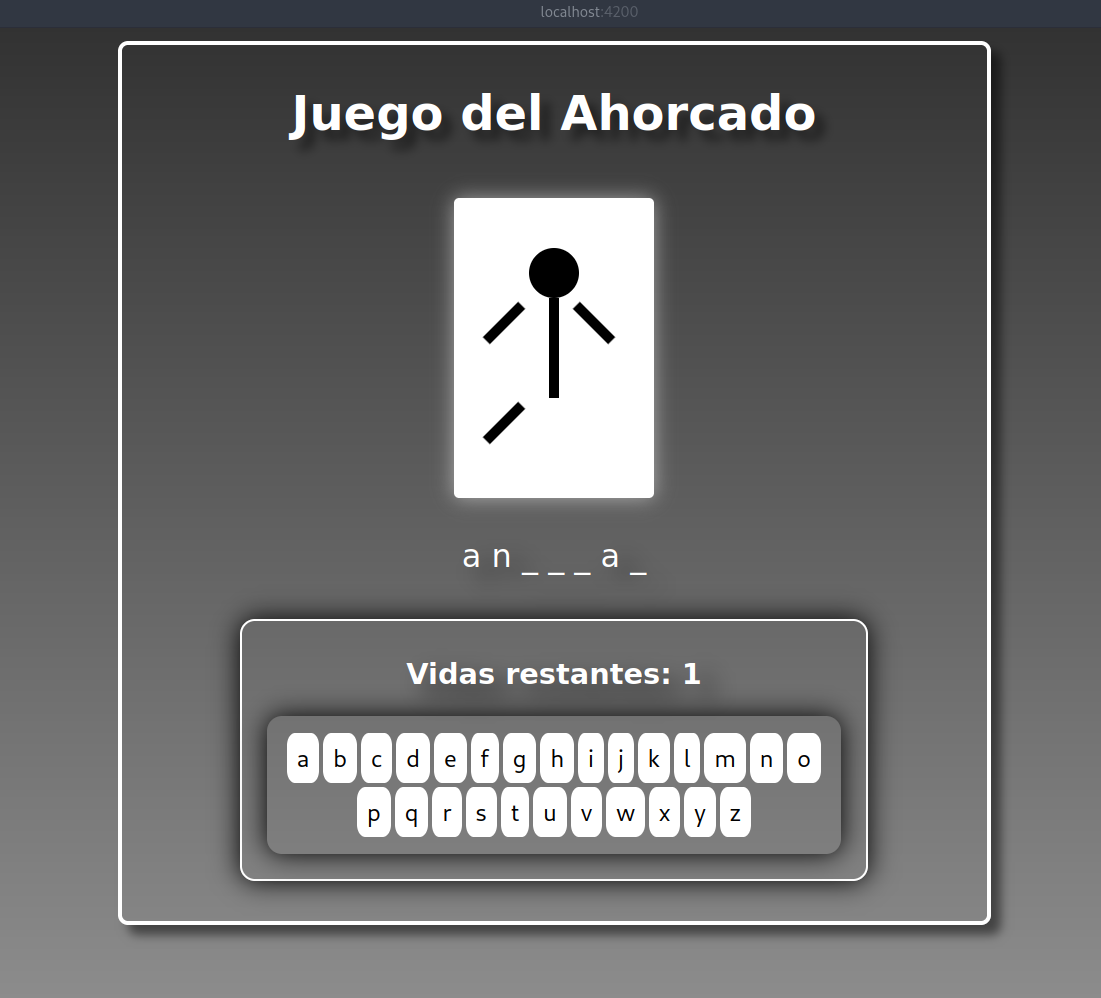
\includegraphics[width=0.8\textwidth]{img/juego_ahorcado.png}
  \caption{Juego del Ahorcado}
\end{figure}


\end{document}
